% Fig. 2 -- teacher->student pipeline with the two losses (Task T5). Plain TikZ, no extra libraries.
% Notation matches Sec. II (Eqs. eq:softmax-T, eq:kd-objective, eq:logit-grads).
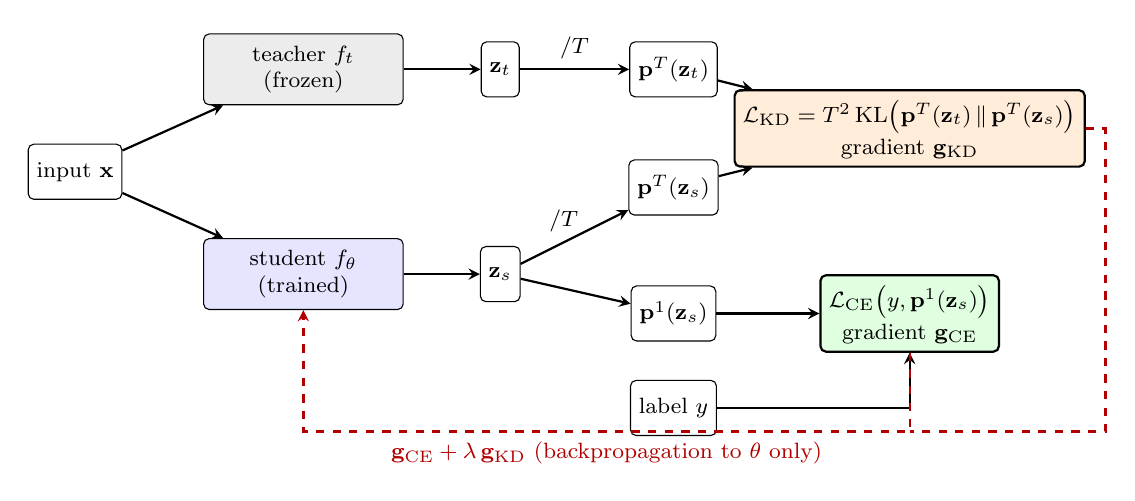
\begin{tikzpicture}[x=1cm, y=1cm, font=\footnotesize, >=stealth,
  net/.style={draw, rounded corners=2pt, align=center, minimum height=0.9cm, text width=2.3cm},
  box/.style={draw, rounded corners=2pt, align=center, minimum height=0.7cm, inner sep=3pt},
  loss/.style={draw, thick, rounded corners=2pt, align=center, minimum height=0.8cm, inner sep=3pt},
  ar/.style={->, thick}]
  \node[box] (x) at (0,0) {input $\mathbf{x}$};
  \node[net, fill=gray!15] (T) at (2.9,1.3) {teacher $f_t$\\(frozen)};
  \node[net, fill=blue!10] (S) at (2.9,-1.3) {student $f_{\theta}$\\(trained)};
  \node[box] (zt) at (5.4,1.3) {$\mathbf{z}_t$};
  \node[box] (zs) at (5.4,-1.3) {$\mathbf{z}_s$};
  \node[box] (pt) at (7.6,1.3) {$\mathbf{p}^{T}(\mathbf{z}_t)$};
  \node[box] (psT) at (7.6,-0.2) {$\mathbf{p}^{T}(\mathbf{z}_s)$};
  \node[box] (ps1) at (7.6,-1.8) {$\mathbf{p}^{1}(\mathbf{z}_s)$};
  \node[loss, fill=orange!15] (Lkd) at (10.6,0.55) {$\mathcal{L}_{\mathrm{KD}}=T^2\,\mathrm{KL}\big(\mathbf{p}^{T}(\mathbf{z}_t)\,\|\,\mathbf{p}^{T}(\mathbf{z}_s)\big)$\\[1pt]gradient $\mathbf{g}_{\mathrm{KD}}$};
  \node[loss, fill=green!12] (Lce) at (10.6,-1.8) {$\mathcal{L}_{\mathrm{CE}}\big(y,\mathbf{p}^{1}(\mathbf{z}_s)\big)$\\[1pt]gradient $\mathbf{g}_{\mathrm{CE}}$};
  \node[box] (y) at (7.6,-3.0) {label $y$};
  \draw[ar] (x) -- (T);
  \draw[ar] (x) -- (S);
  \draw[ar] (T) -- (zt);
  \draw[ar] (S) -- (zs);
  \draw[ar] (zt) -- node[above] {$/T$} (pt);
  \draw[ar] (zs) -- node[above, pos=0.4] {$/T$} (psT);
  \draw[ar] (zs) -- (ps1);
  \draw[ar] (pt) -- (Lkd);
  \draw[ar] (psT) -- (Lkd);
  \draw[ar] (ps1) -- (Lce);
  \draw[ar] (y) -| (Lce);
  % backward pass: only the student receives gradients
  \draw[->, dashed, thick, red!70!black] (Lce.south) -- ++(0,-1.0) -| node[pos=0.25, below] {$\mathbf{g}_{\mathrm{CE}}+\lambda\,\mathbf{g}_{\mathrm{KD}}$ (backpropagation to $\theta$ only)} (S.south);
  \draw[dashed, thick, red!70!black] (Lkd.east) -- ++(0.25,0) |- ([yshift=-1.0cm]Lce.south);
\end{tikzpicture}
